\section{Problem}
\begin{frame}
	\frametitle{Load and production balancing}
	\begin{columns}
		\begin{column}{0.5\textwidth}
				\begin{itemize}
				\item<1-> The power system frequency measures the power balance.
				\item<2-> It is the responsibility of Statnett to control the frequency.
				\item<3-> However, it is the power plant owners who can control the frequency.
			\end{itemize}
		\end{column}
		\begin{column}{0.5\textwidth}
			\begin{figure}
				\includegraphics<1>[width=0.8\textwidth]{./pictures/balance.png}
				\includegraphics<2>[width=0.8\textwidth]{./pictures/balance_statnett.png}
				\includegraphics<3->[width=0.8\textwidth]{./pictures/balance_producers.png}
			\end{figure}
		\end{column}
	\end{columns}
\end{frame}
\begin{frame}
\frametitle{Buying frequency control}
\begin{columns}
\begin{column}{0.5\textwidth}
		\begin{itemize}
		\item<1-> Statnett pays all power plant owners to provide frequency control.
		\item<2-> However, they don't provide the same quality of service.
		\item<3-> Renewable energy sources such as wind and solar don't contribute.

	\end{itemize}
\end{column}
\begin{column}{0.5\textwidth}
	\begin{figure}
		\includegraphics<1>[width=0.8\textwidth]{./pictures/fcp_response_one.tikz}
		\includegraphics<2>[width=0.8\textwidth]{./pictures/fcp_response.tikz}
		\includegraphics<3->[width=0.8\textwidth]{./pictures/res_response.tikz}
		\caption{Frequency control response to step change in frequency}
	\end{figure}
\end{column}
\end{columns}
\end{frame}
\begin{frame}
\frametitle{Future of frequency control}
\begin{columns}
\begin{column}{0.4\textwidth}
		\begin{itemize}
		\item Power plants have to pass tests to get paid to provide frequency control.
		\item Only those who pass the tests get paid for the service.
	\end{itemize}
\end{column}
\begin{column}{0.6\textwidth}
	\begin{figure}
		\includegraphics{./pictures/block.tikz}
		\caption{Test of power plant}
	\end{figure}
\end{column}
\end{columns}
\end{frame}
\begin{frame}
		\frametitle{Tests proposed by the industry}
		\begin{figure}
				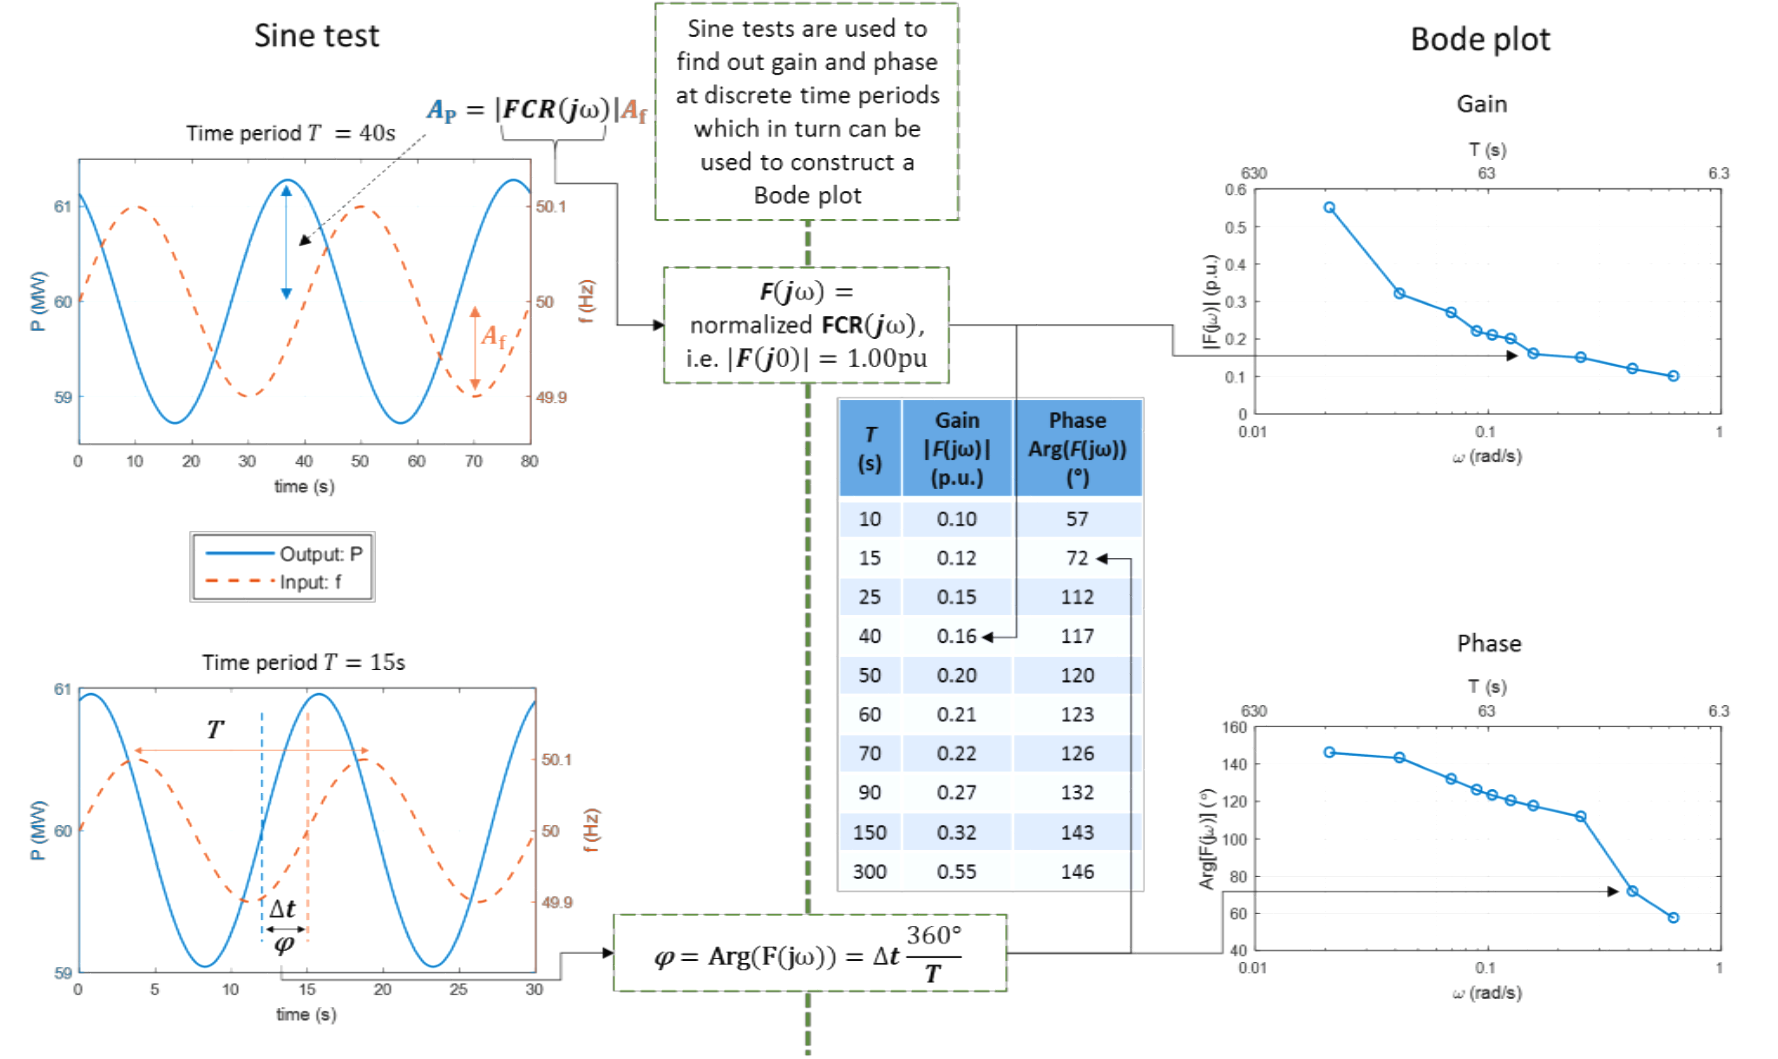
\includegraphics[width=\textwidth]{./pictures/tests.png}
				\caption{Testing procedure [source:ENTSO-E]}
		\end{figure}
\end{frame}
\begin{frame}
		\frametitle{Example from real tests}
		\begin{columns}
				\begin{column}{0.5\textwidth}
						\begin{itemize}
								\item<1-> The power plant needs to be disconnected
								\item<1-> Takes up to 20 hours.
								\item<2-> Only one sine test needed with model learning.
						\end{itemize}
			\end{column}
			\begin{column}{0.5\textwidth}
						\begin{figure}
						\includegraphics<1->[width=\textwidth]{./pictures/aura_signals.tikz}
						\includegraphics<1>[width=\textwidth]{./pictures/frd.tikz}
						\includegraphics<2>[width=\textwidth]{./pictures/frd_vs_bj.tikz}
				\end{figure}
				\end{column}
		\end{columns}
\end{frame}
\begin{frame}
		\frametitle{Motivation}
		\begin{columns}
				\begin{column}{0.5\textwidth}
						\begin{itemize}
								\item<1-> The power system is never really in steady state.
								\item<2-> Can the power plant dynamics be identified from normal operation measurements?
						\end{itemize}
			\end{column}
			\begin{column}{0.5\textwidth}
						\begin{figure}
						\includegraphics<1->[width=\textwidth]{./pictures/aura_pmu.tikz}
				\end{figure}
				\end{column}
		\end{columns}
\end{frame}
\begin{frame}
		\frametitle{Research questions}
		\begin{columns}
				\begin{column}{0.5\textwidth}
						\begin{itemize}
								\item<1-> Can power plant dynamics be identified using a PMU?
								\item<2-> Can power plant dynamics be identified using control system measurements without disturbing the operation of the plant?
								\item<3-> What is the effect of nonlinearities on the identification?

						\end{itemize}
			\end{column}
			\begin{column}{0.5\textwidth}
						\begin{figure}
						\includegraphics<1>[width=\textwidth]{./pictures/aura_pmu.tikz}
						\includegraphics<2>[width=\textwidth]{./pictures/aura_signals.tikz}
						\includegraphics<3>[width=\textwidth]{./pictures/backlash_response.tikz}
				\end{figure}
				\end{column}
		\end{columns}
\end{frame}
